% Options for packages loaded elsewhere
\PassOptionsToPackage{unicode}{hyperref}
\PassOptionsToPackage{hyphens}{url}
%
\documentclass[
]{book}
\usepackage{amsmath,amssymb}
\usepackage{lmodern}
\usepackage{iftex}
\ifPDFTeX
  \usepackage[T1]{fontenc}
  \usepackage[utf8]{inputenc}
  \usepackage{textcomp} % provide euro and other symbols
\else % if luatex or xetex
  \usepackage{unicode-math}
  \defaultfontfeatures{Scale=MatchLowercase}
  \defaultfontfeatures[\rmfamily]{Ligatures=TeX,Scale=1}
\fi
% Use upquote if available, for straight quotes in verbatim environments
\IfFileExists{upquote.sty}{\usepackage{upquote}}{}
\IfFileExists{microtype.sty}{% use microtype if available
  \usepackage[]{microtype}
  \UseMicrotypeSet[protrusion]{basicmath} % disable protrusion for tt fonts
}{}
\makeatletter
\@ifundefined{KOMAClassName}{% if non-KOMA class
  \IfFileExists{parskip.sty}{%
    \usepackage{parskip}
  }{% else
    \setlength{\parindent}{0pt}
    \setlength{\parskip}{6pt plus 2pt minus 1pt}}
}{% if KOMA class
  \KOMAoptions{parskip=half}}
\makeatother
\usepackage{xcolor}
\IfFileExists{xurl.sty}{\usepackage{xurl}}{} % add URL line breaks if available
\IfFileExists{bookmark.sty}{\usepackage{bookmark}}{\usepackage{hyperref}}
\hypersetup{
  pdftitle={RMarkdown automation.},
  pdfauthor={Rachael Remington; Anthony Davidson},
  hidelinks,
  pdfcreator={LaTeX via pandoc}}
\urlstyle{same} % disable monospaced font for URLs
\usepackage{color}
\usepackage{fancyvrb}
\newcommand{\VerbBar}{|}
\newcommand{\VERB}{\Verb[commandchars=\\\{\}]}
\DefineVerbatimEnvironment{Highlighting}{Verbatim}{commandchars=\\\{\}}
% Add ',fontsize=\small' for more characters per line
\usepackage{framed}
\definecolor{shadecolor}{RGB}{248,248,248}
\newenvironment{Shaded}{\begin{snugshade}}{\end{snugshade}}
\newcommand{\AlertTok}[1]{\textcolor[rgb]{0.94,0.16,0.16}{#1}}
\newcommand{\AnnotationTok}[1]{\textcolor[rgb]{0.56,0.35,0.01}{\textbf{\textit{#1}}}}
\newcommand{\AttributeTok}[1]{\textcolor[rgb]{0.77,0.63,0.00}{#1}}
\newcommand{\BaseNTok}[1]{\textcolor[rgb]{0.00,0.00,0.81}{#1}}
\newcommand{\BuiltInTok}[1]{#1}
\newcommand{\CharTok}[1]{\textcolor[rgb]{0.31,0.60,0.02}{#1}}
\newcommand{\CommentTok}[1]{\textcolor[rgb]{0.56,0.35,0.01}{\textit{#1}}}
\newcommand{\CommentVarTok}[1]{\textcolor[rgb]{0.56,0.35,0.01}{\textbf{\textit{#1}}}}
\newcommand{\ConstantTok}[1]{\textcolor[rgb]{0.00,0.00,0.00}{#1}}
\newcommand{\ControlFlowTok}[1]{\textcolor[rgb]{0.13,0.29,0.53}{\textbf{#1}}}
\newcommand{\DataTypeTok}[1]{\textcolor[rgb]{0.13,0.29,0.53}{#1}}
\newcommand{\DecValTok}[1]{\textcolor[rgb]{0.00,0.00,0.81}{#1}}
\newcommand{\DocumentationTok}[1]{\textcolor[rgb]{0.56,0.35,0.01}{\textbf{\textit{#1}}}}
\newcommand{\ErrorTok}[1]{\textcolor[rgb]{0.64,0.00,0.00}{\textbf{#1}}}
\newcommand{\ExtensionTok}[1]{#1}
\newcommand{\FloatTok}[1]{\textcolor[rgb]{0.00,0.00,0.81}{#1}}
\newcommand{\FunctionTok}[1]{\textcolor[rgb]{0.00,0.00,0.00}{#1}}
\newcommand{\ImportTok}[1]{#1}
\newcommand{\InformationTok}[1]{\textcolor[rgb]{0.56,0.35,0.01}{\textbf{\textit{#1}}}}
\newcommand{\KeywordTok}[1]{\textcolor[rgb]{0.13,0.29,0.53}{\textbf{#1}}}
\newcommand{\NormalTok}[1]{#1}
\newcommand{\OperatorTok}[1]{\textcolor[rgb]{0.81,0.36,0.00}{\textbf{#1}}}
\newcommand{\OtherTok}[1]{\textcolor[rgb]{0.56,0.35,0.01}{#1}}
\newcommand{\PreprocessorTok}[1]{\textcolor[rgb]{0.56,0.35,0.01}{\textit{#1}}}
\newcommand{\RegionMarkerTok}[1]{#1}
\newcommand{\SpecialCharTok}[1]{\textcolor[rgb]{0.00,0.00,0.00}{#1}}
\newcommand{\SpecialStringTok}[1]{\textcolor[rgb]{0.31,0.60,0.02}{#1}}
\newcommand{\StringTok}[1]{\textcolor[rgb]{0.31,0.60,0.02}{#1}}
\newcommand{\VariableTok}[1]{\textcolor[rgb]{0.00,0.00,0.00}{#1}}
\newcommand{\VerbatimStringTok}[1]{\textcolor[rgb]{0.31,0.60,0.02}{#1}}
\newcommand{\WarningTok}[1]{\textcolor[rgb]{0.56,0.35,0.01}{\textbf{\textit{#1}}}}
\usepackage{longtable,booktabs,array}
\usepackage{calc} % for calculating minipage widths
% Correct order of tables after \paragraph or \subparagraph
\usepackage{etoolbox}
\makeatletter
\patchcmd\longtable{\par}{\if@noskipsec\mbox{}\fi\par}{}{}
\makeatother
% Allow footnotes in longtable head/foot
\IfFileExists{footnotehyper.sty}{\usepackage{footnotehyper}}{\usepackage{footnote}}
\makesavenoteenv{longtable}
\usepackage{graphicx}
\makeatletter
\def\maxwidth{\ifdim\Gin@nat@width>\linewidth\linewidth\else\Gin@nat@width\fi}
\def\maxheight{\ifdim\Gin@nat@height>\textheight\textheight\else\Gin@nat@height\fi}
\makeatother
% Scale images if necessary, so that they will not overflow the page
% margins by default, and it is still possible to overwrite the defaults
% using explicit options in \includegraphics[width, height, ...]{}
\setkeys{Gin}{width=\maxwidth,height=\maxheight,keepaspectratio}
% Set default figure placement to htbp
\makeatletter
\def\fps@figure{htbp}
\makeatother
\setlength{\emergencystretch}{3em} % prevent overfull lines
\providecommand{\tightlist}{%
  \setlength{\itemsep}{0pt}\setlength{\parskip}{0pt}}
\setcounter{secnumdepth}{5}
\usepackage{booktabs}
\ifLuaTeX
  \usepackage{selnolig}  % disable illegal ligatures
\fi
\usepackage[]{natbib}
\bibliographystyle{plainnat}

\title{RMarkdown automation.}
\usepackage{etoolbox}
\makeatletter
\providecommand{\subtitle}[1]{% add subtitle to \maketitle
  \apptocmd{\@title}{\par {\large #1 \par}}{}{}
}
\makeatother
\subtitle{Extending research into application}
\author{Rachael Remington; Anthony Davidson}
\date{2022-05-17}

\begin{document}
\maketitle

{
\setcounter{tocdepth}{1}
\tableofcontents
}
\hypertarget{index}{%
\chapter{index}\label{index}}

ss.

Last week we began to set up our projects using RMarkdown and R code so that we are ready for Terry Newmans sample/survey design session.

Now this is postponed till next week we can finish this off.

\hypertarget{rstudio-project-file}{%
\chapter{RStudio project file}\label{rstudio-project-file}}

\begin{itemize}
\tightlist
\item
  \url{https://r4ds.had.co.nz/workflow-projects.html}
\end{itemize}

\hypertarget{git-ignore-file}{%
\section{git ignore file}\label{git-ignore-file}}

\begin{verbatim}
# History files
.Rhistory
.Rapp.history

# Session Data files
.RData

# User-specific files
.Ruserdata

# Example code in package build process
*-Ex.R

# Output files from R CMD build
/*.tar.gz

# Output files from R CMD check
/*.Rcheck/

# RStudio files
.Rproj.user/

# produced vignettes
vignettes/*.html
vignettes/*.pdf

# OAuth2 token, see https://github.com/hadley/httr/releases/tag/v0.3
.httr-oauth

# knitr and R markdown default cache directories
*_cache/
/cache/

# Temporary files created by R markdown
*.utf8.md
*.knit.md

# R Environment Variables
.Renviron

#notes
/notes2022/
/_main/
/libs/
/experimental_plan/
/Presentation/
/data/
\end{verbatim}

\hypertarget{biol8700_setup_2022}{%
\chapter{BIOL8700\_setup\_2022}\label{biol8700_setup_2022}}

The goal of BIOL8700\_setup\_2022 is to setup and generate documents using RStudio, RMarkdown and github

\hypertarget{tools}{%
\section{Tools}\label{tools}}

This is a \emph{sample} book written in \textbf{Markdown} and includes embedded R code. This combination of programming languages is included in the RMarkdown package. We use this and a variation of other RMarkdown packages to make the most of reproducible reporting in R.

\hypertarget{data-importing}{%
\section{Data importing}\label{data-importing}}

There are scripts and code included within this repository to import data from csv and excel files from local and online locations.

\hypertarget{results}{%
\section{Results}\label{results}}

You can also embed plots, code and data in an RMarkdown document. The core results of this repository are as follows:

In that case, don't forget to commit and push the resulting figure files, so they display on GitHub.

\hypertarget{quick-overview-of-last-week}{%
\subsection{Quick overview of last week}\label{quick-overview-of-last-week}}

\begin{enumerate}
\def\labelenumi{\arabic{enumi}.}
\tightlist
\item
  Run the R chunk below and check that you have all the packages running from last week.
\end{enumerate}

\begin{Shaded}
\begin{Highlighting}[]
\FunctionTok{library}\NormalTok{(rmarkdown)}
\FunctionTok{library}\NormalTok{(rticles)}
\FunctionTok{library}\NormalTok{(bookdown)}
\FunctionTok{library}\NormalTok{(bookdownplus)}
\FunctionTok{library}\NormalTok{(tidyverse)}
\CommentTok{\#\textgreater{} {-}{-} Attaching packages {-}{-}{-}{-}{-}{-}{-}{-}{-}{-}{-}{-}{-}{-}{-}{-}{-}{-}{-}{-}{-}{-}{-}{-}{-}{-}{-}{-}{-}{-}{-}{-}{-}{-}{-}{-}{-}{-}{-} tidyverse 1.3.1 {-}{-}}
\CommentTok{\#\textgreater{} v ggplot2 3.3.5     v purrr   0.3.4}
\CommentTok{\#\textgreater{} v tibble  3.1.6     v dplyr   1.0.8}
\CommentTok{\#\textgreater{} v tidyr   1.2.0     v stringr 1.4.0}
\CommentTok{\#\textgreater{} v readr   2.1.2     v forcats 0.5.1}
\CommentTok{\#\textgreater{} {-}{-} Conflicts {-}{-}{-}{-}{-}{-}{-}{-}{-}{-}{-}{-}{-}{-}{-}{-}{-}{-}{-}{-}{-}{-}{-}{-}{-}{-}{-}{-}{-}{-}{-}{-}{-}{-}{-}{-}{-}{-}{-}{-}{-}{-} tidyverse\_conflicts() {-}{-}}
\CommentTok{\#\textgreater{} x dplyr::filter() masks stats::filter()}
\CommentTok{\#\textgreater{} x dplyr::lag()    masks stats::lag()}
\FunctionTok{library}\NormalTok{(readxl)}
\end{Highlighting}
\end{Shaded}

\begin{enumerate}
\def\labelenumi{\arabic{enumi}.}
\setcounter{enumi}{1}
\tightlist
\item
  Can you import the data set you found last week in class?
\end{enumerate}

\begin{Shaded}
\begin{Highlighting}[]
\CommentTok{\#read.csv}
\CommentTok{\#read.xl}
\CommentTok{\#example from }
\end{Highlighting}
\end{Shaded}

\begin{itemize}
\tightlist
\item
  What options did we have?
\item
  Here I will take the following dataset and extend this to include some code and plots for the data
\end{itemize}

\begin{enumerate}
\def\labelenumi{\arabic{enumi}.}
\setcounter{enumi}{2}
\item
  Follow along with the next chapter\ldots.
\item
\end{enumerate}

\begin{Shaded}
\begin{Highlighting}[]
\FunctionTok{library}\NormalTok{(tidyverse)}
\FunctionTok{library}\NormalTok{(jtools)}
\end{Highlighting}
\end{Shaded}

\hypertarget{experimental-plan-template}{%
\chapter{Experimental plan template}\label{experimental-plan-template}}

Now that you have been developing a research question over the last few months, the next step is to design a set of experiments that will specifically test your research aims.

We are often focused on the ``cookbook'' aspect of experiments -- the protocols and steps required to conduct each experiment. However, it's critical to spend time designing your overall experimental approach and the finer details to ensure that your research will produce robust data that can be clearly analysed without bias. When we test specific questions, we want to avoid statistical issues such as ``noise'' and ``confounding'' factors.

Terry Neeman will be delivering a workshop to help you strengthen your experimental plan -- both in terms of your proposed design, and to help you more clearly and accurately explain the rationale and set-up of your experiments. This workshop will help you apply the principles taught in BIOL8291 to your own experiment. To prepare, you will create an outline of your experimental plan, focusing on the statistical framework of your design.

Below is an outline of questions for you to answer/justify for each part of your experimental plan. You will also need to draw two figures (digital drawings preferred) for each aim that show:

\begin{enumerate}
\def\labelenumi{\arabic{enumi})}
\item
  a simple overview of the experimental plan related to the research aim,
\item
  a detailed ``snap-shot'' of the experimental set up (i.e., how will the plates, plants, etc. be arranged? Will there be a row-column design? Blocking? Randomization? What treatments will be applied and how many replicates will be tested?)
\end{enumerate}

You can access the template for the experimental plan on Wattle or a copy can be found within this repository. \href{\%223.\%20Statistical\%20Methods\%20in\%20Biology\%20-\%20Chapter\%203.pdf\%22}{DOWNLOAD NOW}. The template is laid out below as follows:

\hypertarget{research-questions}{%
\section{Research Question(s)?}\label{research-questions}}

\begin{Shaded}
\begin{Highlighting}[]
\CommentTok{\#input question here}
\end{Highlighting}
\end{Shaded}

\hypertarget{experimental-aims}{%
\section{Experimental Aims?}\label{experimental-aims}}

For each experiment explain the overall experimental approach (1-3 sentences + overview diagram) list:

\begin{enumerate}
\def\labelenumi{\arabic{enumi})}
\tightlist
\item
  the response variables/outcome measure(s) for the experiment
\item
  the experimental factor(s) of interest
\item
  the experimental conditions (groups for comparisons), and the number of replicates/sample size for each condition
\item
  the experimental control(s)
\item
  are their any potentially confounding factors (``nuisance factors'')? Briefly explain how they will be tracked/or mitigated
\end{enumerate}

Briefly explain the design of the experiment and provide a diagram that shows a ``snap shot'' of the experimental set-up (e.g., how all the plants under different experimental conditions will be arranged, all the plates in the lab, a flow chart of computational steps, etc.). Make sure to consider and include relevant design aspects like blocking, randomisation, as well as to clearly indicate treatments, replicate numbers, and controls.

\begin{quote}
TIP: Start thinking about how you will analyse your data:\\
``what statistical tests would you use?''
\end{quote}

\hypertarget{importing-data}{%
\subsubsection{Importing data}\label{importing-data}}

\hypertarget{visualising-data}{%
\subsubsection{Visualising data}\label{visualising-data}}

\hypertarget{reporting}{%
\subsubsection{Reporting}\label{reporting}}

\hypertarget{rmarkdown-reports}{%
\chapter{RMarkdown reports}\label{rmarkdown-reports}}

We should all know what these are and how to render a report in RMarkdown. Next we will produce a RMarkdown document for the question we have been working on ready to add data and other sampling design information.

\begin{Shaded}
\begin{Highlighting}[]
\CommentTok{\#general packages used}
\FunctionTok{library}\NormalTok{(tidyverse)}
\end{Highlighting}
\end{Shaded}

What does this tell us about how RProjects and other funky things work?

\begin{enumerate}
\def\labelenumi{\arabic{enumi}.}
\setcounter{enumi}{2}
\tightlist
\item
  Data import
\end{enumerate}

\begin{Shaded}
\begin{Highlighting}[]
\NormalTok{dat }\OtherTok{\textless{}{-}} \FunctionTok{read.csv}\NormalTok{(}\StringTok{"data/Analysis\_ardMods.csv"}\NormalTok{)}
\FunctionTok{glimpse}\NormalTok{(dat)}
\CommentTok{\#\textgreater{} Rows: 380}
\CommentTok{\#\textgreater{} Columns: 35}
\CommentTok{\#\textgreater{} $ Well                   \textless{}chr\textgreater{} "1", "2", "3", "4", "5", "6", "7", "8", "9", "1\textasciitilde{}}
\CommentTok{\#\textgreater{} $ Well.Position          \textless{}chr\textgreater{} "A1", "A2", "A3", "A4", "A5", "A6", "A7", "A8",\textasciitilde{}}
\CommentTok{\#\textgreater{} $ Omit                   \textless{}chr\textgreater{} "false", "false", "false", "false", "false", "f\textasciitilde{}}
\CommentTok{\#\textgreater{} $ Sample.Name            \textless{}chr\textgreater{} "1", "2", "3", "4", "5", "6", "7", "8", "9", "1\textasciitilde{}}
\CommentTok{\#\textgreater{} $ Delta.Ct.SE            \textless{}lgl\textgreater{} NA, NA, NA, NA, NA, NA, NA, NA, NA, NA, NA, NA,\textasciitilde{}}
\CommentTok{\#\textgreater{} $ Target.Name            \textless{}chr\textgreater{} "Gapdh", "Gapdh", "Gapdh", "Gapdh", "Gapdh", "G\textasciitilde{}}
\CommentTok{\#\textgreater{} $ Task                   \textless{}chr\textgreater{} "UNKNOWN", "UNKNOWN", "UNKNOWN", "UNKNOWN", "UN\textasciitilde{}}
\CommentTok{\#\textgreater{} $ Reporter               \textless{}chr\textgreater{} "SYBR", "SYBR", "SYBR", "SYBR", "SYBR", "SYBR",\textasciitilde{}}
\CommentTok{\#\textgreater{} $ Quencher               \textless{}chr\textgreater{} "None", "None", "None", "None", "None", "None",\textasciitilde{}}
\CommentTok{\#\textgreater{} $ RQ                     \textless{}dbl\textgreater{} NA, NA, NA, NA, NA, NA, NA, NA, NA, NA, NA, NA,\textasciitilde{}}
\CommentTok{\#\textgreater{} $ RQ.Min                 \textless{}dbl\textgreater{} NA, NA, NA, NA, NA, NA, NA, NA, NA, NA, NA, NA,\textasciitilde{}}
\CommentTok{\#\textgreater{} $ RQ.Max                 \textless{}dbl\textgreater{} NA, NA, NA, NA, NA, NA, NA, NA, NA, NA, NA, NA,\textasciitilde{}}
\CommentTok{\#\textgreater{} $ CT                     \textless{}chr\textgreater{} "12.909", "14.253", "13.532", "13.377", "14.249\textasciitilde{}}
\CommentTok{\#\textgreater{} $ EQ.Ct.Mean             \textless{}dbl\textgreater{} 12.909, 14.253, 13.532, 13.377, 14.249, 15.053,\textasciitilde{}}
\CommentTok{\#\textgreater{} $ EQ.Ct.SE               \textless{}lgl\textgreater{} NA, NA, NA, NA, NA, NA, NA, NA, NA, NA, NA, NA,\textasciitilde{}}
\CommentTok{\#\textgreater{} $ Quantity               \textless{}lgl\textgreater{} NA, NA, NA, NA, NA, NA, NA, NA, NA, NA, NA, NA,\textasciitilde{}}
\CommentTok{\#\textgreater{} $ Delta.Ct.Mean          \textless{}dbl\textgreater{} NA, NA, NA, NA, NA, NA, NA, NA, NA, NA, NA, NA,\textasciitilde{}}
\CommentTok{\#\textgreater{} $ Delta.Delta.Ct         \textless{}dbl\textgreater{} NA, NA, NA, NA, NA, NA, NA, NA, NA, NA, NA, NA,\textasciitilde{}}
\CommentTok{\#\textgreater{} $ Automatic.Ct.Threshold \textless{}chr\textgreater{} "true", "true", "true", "true", "true", "true",\textasciitilde{}}
\CommentTok{\#\textgreater{} $ Ct.Threshold           \textless{}dbl\textgreater{} 0.062, 0.062, 0.062, 0.062, 0.062, 0.062, 0.062\textasciitilde{}}
\CommentTok{\#\textgreater{} $ Automatic.Baseline     \textless{}chr\textgreater{} "true", "true", "true", "true", "true", "true",\textasciitilde{}}
\CommentTok{\#\textgreater{} $ Baseline.Start         \textless{}int\textgreater{} 3, 3, 3, 3, 3, 3, 3, 3, 3, 3, 3, 3, 3, 3, 3, 3,\textasciitilde{}}
\CommentTok{\#\textgreater{} $ Baseline.End           \textless{}int\textgreater{} 9, 11, 10, 10, 11, 13, 10, 10, 11, 10, 9, 9, 10\textasciitilde{}}
\CommentTok{\#\textgreater{} $ Efficiency             \textless{}lgl\textgreater{} NA, NA, NA, NA, NA, NA, NA, NA, NA, NA, NA, NA,\textasciitilde{}}
\CommentTok{\#\textgreater{} $ Tm1                    \textless{}dbl\textgreater{} 84.395, 84.395, 84.395, 84.395, 84.395, 84.527,\textasciitilde{}}
\CommentTok{\#\textgreater{} $ Comments               \textless{}lgl\textgreater{} NA, NA, NA, NA, NA, NA, NA, NA, NA, NA, NA, NA,\textasciitilde{}}
\CommentTok{\#\textgreater{} $ Tm2                    \textless{}dbl\textgreater{} NA, NA, NA, NA, NA, NA, NA, NA, NA, NA, NA, NA,\textasciitilde{}}
\CommentTok{\#\textgreater{} $ Amp.Score              \textless{}dbl\textgreater{} 1.346, 1.345, 1.352, 1.349, 1.339, 1.356, 1.347\textasciitilde{}}
\CommentTok{\#\textgreater{} $ Tm3                    \textless{}dbl\textgreater{} NA, NA, NA, NA, NA, NA, NA, NA, NA, NA, NA, NA,\textasciitilde{}}
\CommentTok{\#\textgreater{} $ Cq.Conf                \textless{}dbl\textgreater{} 0.920, 0.872, 0.930, 0.933, 0.974, 0.938, 0.924\textasciitilde{}}
\CommentTok{\#\textgreater{} $ MTP                    \textless{}chr\textgreater{} "N", "N", "N", "N", "N", "N", "N", "N", "N", "N\textasciitilde{}}
\CommentTok{\#\textgreater{} $ EXPFAIL                \textless{}chr\textgreater{} "N", "N", "N", "N", "N", "N", "N", "N", "N", "N\textasciitilde{}}
\CommentTok{\#\textgreater{} $ NOISE                  \textless{}chr\textgreater{} "N", "N", "N", "N", "N", "N", "N", "N", "N", "N\textasciitilde{}}
\CommentTok{\#\textgreater{} $ NOAMP                  \textless{}chr\textgreater{} "N", "N", "N", "N", "N", "N", "N", "N", "N", "N\textasciitilde{}}
\CommentTok{\#\textgreater{} $ THOLDFAIL              \textless{}chr\textgreater{} "N", "N", "N", "N", "N", "N", "N", "N", "N", "N\textasciitilde{}}
\end{Highlighting}
\end{Shaded}

\begin{enumerate}
\def\labelenumi{\arabic{enumi}.}
\setcounter{enumi}{3}
\tightlist
\item
  Data visualisation
\end{enumerate}

\begin{Shaded}
\begin{Highlighting}[]
\CommentTok{\# table(dat$Well.Position)}
\FunctionTok{mean}\NormalTok{(dat}\SpecialCharTok{$}\NormalTok{Delta.Ct.Mean, }\AttributeTok{na.rm =} \ConstantTok{TRUE}\NormalTok{)}
\CommentTok{\#\textgreater{} [1] 13.08628}
\FunctionTok{sd}\NormalTok{(dat}\SpecialCharTok{$}\NormalTok{Delta.Ct.Mean, }\AttributeTok{na.rm =} \ConstantTok{TRUE}\NormalTok{)}
\CommentTok{\#\textgreater{} [1] 5.507596}

\FunctionTok{hist}\NormalTok{(dat}\SpecialCharTok{$}\NormalTok{Delta.Ct.Mean)}
\end{Highlighting}
\end{Shaded}

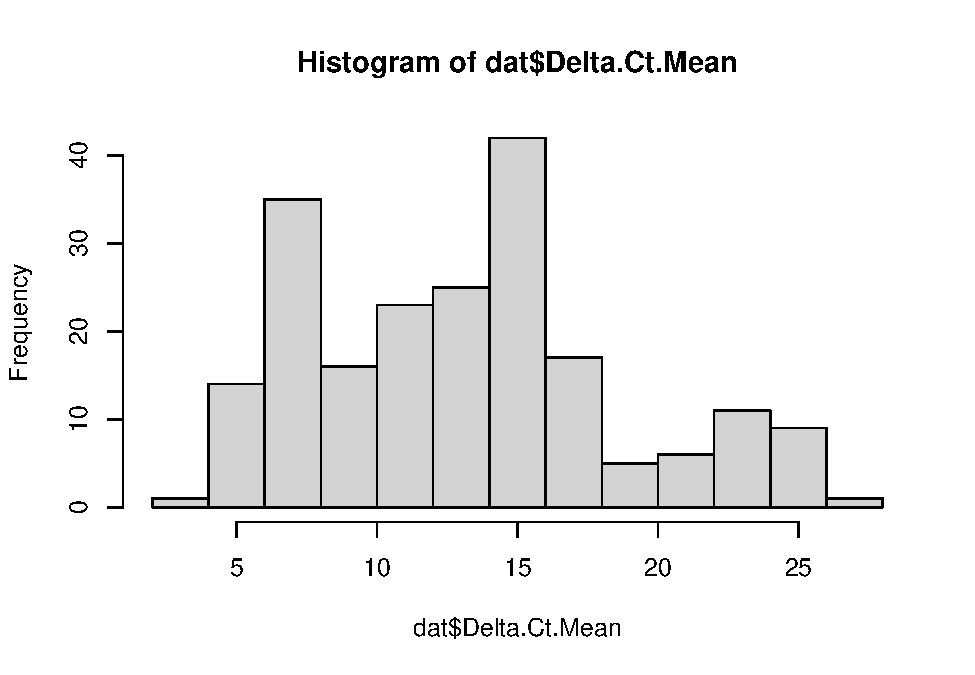
\includegraphics{_main_files/figure-latex/unnamed-chunk-12-1.pdf}

\begin{enumerate}
\def\labelenumi{\arabic{enumi}.}
\setcounter{enumi}{4}
\item
  Tidyverse approach
\item
  ggplot
\end{enumerate}

Tasks ready for next week:

\begin{enumerate}
\def\labelenumi{\arabic{enumi}.}
\item
  Outcome and predictor variables
\item
  Other studies with same sampling design
\item
  Other reference material.
\item
  Read a cool sampling design/issue paper
\end{enumerate}

Watch this short (ish video) as a summary of what you should understand so far.

\hypertarget{sampling-design}{%
\chapter{Sampling design}\label{sampling-design}}

\begin{Shaded}
\begin{Highlighting}[]
\CommentTok{\#general packages used}
\FunctionTok{library}\NormalTok{(tidyverse)}
\FunctionTok{library}\NormalTok{(knitr)}
\end{Highlighting}
\end{Shaded}

We should all know what these are and how to render a report in RMarkdown. Next we will produce a RMarkdown document for the question we have been working on ready to add data and other sampling design information.

\begin{enumerate}
\def\labelenumi{\arabic{enumi}.}
\tightlist
\item
  Outcome and predictor variables
\item
  Other study examples and code
\item
  Other studies with same sampling design
\item
  Other reference material.
\item
  Read a cool sampling design/issue paper
\end{enumerate}

\hypertarget{terrys-lecture-in-rmarkdown}{%
\section{Terry's lecture in RMarkdown}\label{terrys-lecture-in-rmarkdown}}

\begin{Shaded}
\begin{Highlighting}[]
\NormalTok{knitr}\SpecialCharTok{::}\FunctionTok{include\_graphics}\NormalTok{(}\StringTok{"study\_design/Experimental{-}plan{-}workshop Terry Neeman 17 May 2002.pdf"}\NormalTok{)}
\end{Highlighting}
\end{Shaded}


\includegraphics{study_design/Experimental-plan-workshop Terry Neeman 17 May 2002.pdf}

\begin{Shaded}
\begin{Highlighting}[]
\CommentTok{\#general packages used}
\FunctionTok{library}\NormalTok{(tidyverse)}
\end{Highlighting}
\end{Shaded}

\hypertarget{automation}{%
\chapter{Automation}\label{automation}}

What is special about using \texttt{README.Rmd} instead of just \texttt{README.md}?

You can include R chunks like so:

You'll still need to render \texttt{README.Rmd} regularly, to keep \texttt{README.md} up-to-date. \texttt{devtools::build\_readme()} is handy for this. You could also use GitHub Actions to re-render \texttt{README.Rmd} every time you push. An example workflow can be found here: \url{https://github.com/r-lib/actions/tree/v1/examples}.

\hypertarget{rmarkdown-reports-1}{%
\section{RMarkdown reports}\label{rmarkdown-reports-1}}

We should all know what these are and how to render a report in RMarkdown. Next we will produce a RMarkdown document for the question we have been working on ready to add data and other sampling design information.

\begin{enumerate}
\def\labelenumi{\arabic{enumi}.}
\tightlist
\item
  Outcome and predictor variables
\item
  Other study examples and code
\item
  Other studies with same sampling design
\item
  Other reference material.
\item
  Read a cool sampling design/issue paper
\end{enumerate}

Watch this short (ish video) as a summary of what you should understand so far.

What does this tell us about how RProjects and other funky things work?

\begin{enumerate}
\def\labelenumi{\arabic{enumi}.}
\setcounter{enumi}{2}
\tightlist
\item
  Data import
\end{enumerate}

\begin{Shaded}
\begin{Highlighting}[]
\NormalTok{dat }\OtherTok{\textless{}{-}} \FunctionTok{read.csv}\NormalTok{(}\StringTok{"data/Analysis\_ardMods.csv"}\NormalTok{)}
\end{Highlighting}
\end{Shaded}

\begin{enumerate}
\def\labelenumi{\arabic{enumi}.}
\setcounter{enumi}{3}
\tightlist
\item
  Data visualisation
\end{enumerate}

\begin{Shaded}
\begin{Highlighting}[]
\CommentTok{\# table(dat$Well.Position)}
\FunctionTok{mean}\NormalTok{(dat}\SpecialCharTok{$}\NormalTok{Delta.Ct.Mean, }\AttributeTok{na.rm =} \ConstantTok{TRUE}\NormalTok{)}
\CommentTok{\#\textgreater{} [1] 13.08628}
\FunctionTok{sd}\NormalTok{(dat}\SpecialCharTok{$}\NormalTok{Delta.Ct.Mean, }\AttributeTok{na.rm =} \ConstantTok{TRUE}\NormalTok{)}
\CommentTok{\#\textgreater{} [1] 5.507596}

\FunctionTok{hist}\NormalTok{(dat}\SpecialCharTok{$}\NormalTok{Delta.Ct.Mean)}
\end{Highlighting}
\end{Shaded}

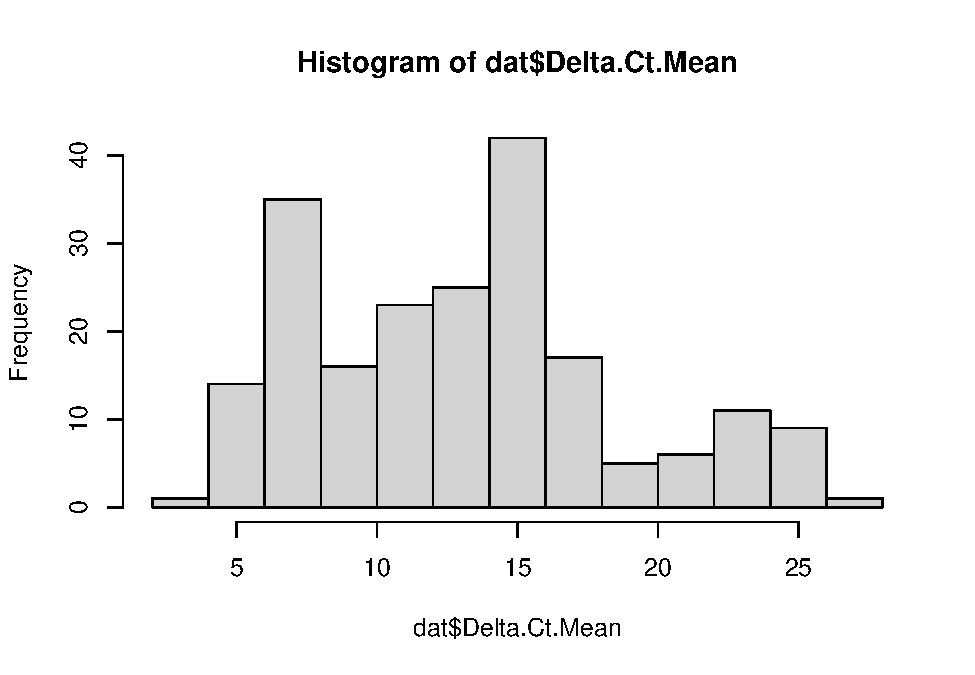
\includegraphics{_main_files/figure-latex/unnamed-chunk-17-1.pdf}

\begin{enumerate}
\def\labelenumi{\arabic{enumi}.}
\setcounter{enumi}{4}
\tightlist
\item
  Tidyverse approach
\end{enumerate}

\begin{Shaded}
\begin{Highlighting}[]
\FunctionTok{glimpse}\NormalTok{(dat)}
\CommentTok{\#\textgreater{} Rows: 380}
\CommentTok{\#\textgreater{} Columns: 35}
\CommentTok{\#\textgreater{} $ Well                   \textless{}chr\textgreater{} "1", "2", "3", "4", "5", "6", "7", "8", "9", "1\textasciitilde{}}
\CommentTok{\#\textgreater{} $ Well.Position          \textless{}chr\textgreater{} "A1", "A2", "A3", "A4", "A5", "A6", "A7", "A8",\textasciitilde{}}
\CommentTok{\#\textgreater{} $ Omit                   \textless{}chr\textgreater{} "false", "false", "false", "false", "false", "f\textasciitilde{}}
\CommentTok{\#\textgreater{} $ Sample.Name            \textless{}chr\textgreater{} "1", "2", "3", "4", "5", "6", "7", "8", "9", "1\textasciitilde{}}
\CommentTok{\#\textgreater{} $ Delta.Ct.SE            \textless{}lgl\textgreater{} NA, NA, NA, NA, NA, NA, NA, NA, NA, NA, NA, NA,\textasciitilde{}}
\CommentTok{\#\textgreater{} $ Target.Name            \textless{}chr\textgreater{} "Gapdh", "Gapdh", "Gapdh", "Gapdh", "Gapdh", "G\textasciitilde{}}
\CommentTok{\#\textgreater{} $ Task                   \textless{}chr\textgreater{} "UNKNOWN", "UNKNOWN", "UNKNOWN", "UNKNOWN", "UN\textasciitilde{}}
\CommentTok{\#\textgreater{} $ Reporter               \textless{}chr\textgreater{} "SYBR", "SYBR", "SYBR", "SYBR", "SYBR", "SYBR",\textasciitilde{}}
\CommentTok{\#\textgreater{} $ Quencher               \textless{}chr\textgreater{} "None", "None", "None", "None", "None", "None",\textasciitilde{}}
\CommentTok{\#\textgreater{} $ RQ                     \textless{}dbl\textgreater{} NA, NA, NA, NA, NA, NA, NA, NA, NA, NA, NA, NA,\textasciitilde{}}
\CommentTok{\#\textgreater{} $ RQ.Min                 \textless{}dbl\textgreater{} NA, NA, NA, NA, NA, NA, NA, NA, NA, NA, NA, NA,\textasciitilde{}}
\CommentTok{\#\textgreater{} $ RQ.Max                 \textless{}dbl\textgreater{} NA, NA, NA, NA, NA, NA, NA, NA, NA, NA, NA, NA,\textasciitilde{}}
\CommentTok{\#\textgreater{} $ CT                     \textless{}chr\textgreater{} "12.909", "14.253", "13.532", "13.377", "14.249\textasciitilde{}}
\CommentTok{\#\textgreater{} $ EQ.Ct.Mean             \textless{}dbl\textgreater{} 12.909, 14.253, 13.532, 13.377, 14.249, 15.053,\textasciitilde{}}
\CommentTok{\#\textgreater{} $ EQ.Ct.SE               \textless{}lgl\textgreater{} NA, NA, NA, NA, NA, NA, NA, NA, NA, NA, NA, NA,\textasciitilde{}}
\CommentTok{\#\textgreater{} $ Quantity               \textless{}lgl\textgreater{} NA, NA, NA, NA, NA, NA, NA, NA, NA, NA, NA, NA,\textasciitilde{}}
\CommentTok{\#\textgreater{} $ Delta.Ct.Mean          \textless{}dbl\textgreater{} NA, NA, NA, NA, NA, NA, NA, NA, NA, NA, NA, NA,\textasciitilde{}}
\CommentTok{\#\textgreater{} $ Delta.Delta.Ct         \textless{}dbl\textgreater{} NA, NA, NA, NA, NA, NA, NA, NA, NA, NA, NA, NA,\textasciitilde{}}
\CommentTok{\#\textgreater{} $ Automatic.Ct.Threshold \textless{}chr\textgreater{} "true", "true", "true", "true", "true", "true",\textasciitilde{}}
\CommentTok{\#\textgreater{} $ Ct.Threshold           \textless{}dbl\textgreater{} 0.062, 0.062, 0.062, 0.062, 0.062, 0.062, 0.062\textasciitilde{}}
\CommentTok{\#\textgreater{} $ Automatic.Baseline     \textless{}chr\textgreater{} "true", "true", "true", "true", "true", "true",\textasciitilde{}}
\CommentTok{\#\textgreater{} $ Baseline.Start         \textless{}int\textgreater{} 3, 3, 3, 3, 3, 3, 3, 3, 3, 3, 3, 3, 3, 3, 3, 3,\textasciitilde{}}
\CommentTok{\#\textgreater{} $ Baseline.End           \textless{}int\textgreater{} 9, 11, 10, 10, 11, 13, 10, 10, 11, 10, 9, 9, 10\textasciitilde{}}
\CommentTok{\#\textgreater{} $ Efficiency             \textless{}lgl\textgreater{} NA, NA, NA, NA, NA, NA, NA, NA, NA, NA, NA, NA,\textasciitilde{}}
\CommentTok{\#\textgreater{} $ Tm1                    \textless{}dbl\textgreater{} 84.395, 84.395, 84.395, 84.395, 84.395, 84.527,\textasciitilde{}}
\CommentTok{\#\textgreater{} $ Comments               \textless{}lgl\textgreater{} NA, NA, NA, NA, NA, NA, NA, NA, NA, NA, NA, NA,\textasciitilde{}}
\CommentTok{\#\textgreater{} $ Tm2                    \textless{}dbl\textgreater{} NA, NA, NA, NA, NA, NA, NA, NA, NA, NA, NA, NA,\textasciitilde{}}
\CommentTok{\#\textgreater{} $ Amp.Score              \textless{}dbl\textgreater{} 1.346, 1.345, 1.352, 1.349, 1.339, 1.356, 1.347\textasciitilde{}}
\CommentTok{\#\textgreater{} $ Tm3                    \textless{}dbl\textgreater{} NA, NA, NA, NA, NA, NA, NA, NA, NA, NA, NA, NA,\textasciitilde{}}
\CommentTok{\#\textgreater{} $ Cq.Conf                \textless{}dbl\textgreater{} 0.920, 0.872, 0.930, 0.933, 0.974, 0.938, 0.924\textasciitilde{}}
\CommentTok{\#\textgreater{} $ MTP                    \textless{}chr\textgreater{} "N", "N", "N", "N", "N", "N", "N", "N", "N", "N\textasciitilde{}}
\CommentTok{\#\textgreater{} $ EXPFAIL                \textless{}chr\textgreater{} "N", "N", "N", "N", "N", "N", "N", "N", "N", "N\textasciitilde{}}
\CommentTok{\#\textgreater{} $ NOISE                  \textless{}chr\textgreater{} "N", "N", "N", "N", "N", "N", "N", "N", "N", "N\textasciitilde{}}
\CommentTok{\#\textgreater{} $ NOAMP                  \textless{}chr\textgreater{} "N", "N", "N", "N", "N", "N", "N", "N", "N", "N\textasciitilde{}}
\CommentTok{\#\textgreater{} $ THOLDFAIL              \textless{}chr\textgreater{} "N", "N", "N", "N", "N", "N", "N", "N", "N", "N\textasciitilde{}}
\end{Highlighting}
\end{Shaded}

\begin{enumerate}
\def\labelenumi{\arabic{enumi}.}
\setcounter{enumi}{5}
\tightlist
\item
  Nicer plots using \texttt{ggplot}
\end{enumerate}

\hypertarget{next-steps}{%
\subsubsection{Next steps}\label{next-steps}}

One aspect that can be challenging when working with RMarkdown documents for manuscripts is references.

The references for a bookdown or rmarkdown file can be included using the following information in the \texttt{yml} header of the index file.
The references for a bookdown or rmarkdown file can be included using the following information in the yml header of the index file.

\begin{verbatim}
\end{verbatim}

\hypertarget{manual-references}{%
\section{Manual references}\label{manual-references}}

\hypertarget{packages}{%
\section{Packages}\label{packages}}

The goal of BIOL877\_setup\_2022 repository here is to provide a starting point for using RMarkdown and RStudio to undertake research.

\hypertarget{download-project-and-files}{%
\section{Download project and files}\label{download-project-and-files}}

We checked and loaded an RMarkdown

This is a \emph{sample} book written in \textbf{Markdown} and extended from the original RMD file. You can use anything that Pandoc's Markdown supports; for example, a math equation \(a^2 + b^2 = c^2\).

\hypertarget{usage}{%
\section{Usage}\label{usage}}

Each \textbf{bookdown} chapter is an .Rmd file, and each .Rmd file can contain one (and only one) chapter. A chapter \emph{must} start with a first-level heading: \texttt{\#\ A\ good\ chapter}, and can contain one (and only one) first-level heading.

Use second-level and higher headings within chapters like: \texttt{\#\#\ A\ short\ section} or \texttt{\#\#\#\ An\ even\ shorter\ section}.

The \texttt{index.Rmd} file is required, and is also your first book chapter. It will be the homepage when you render the book.

\hypertarget{render-book}{%
\section{Render book}\label{render-book}}

You can render the HTML version of this example book without changing anything:

\begin{enumerate}
\def\labelenumi{\arabic{enumi}.}
\item
  Find the \textbf{Build} pane in the RStudio IDE, and
\item
  Click on \textbf{Build Book}, then select your output format, or select ``All formats'' if you'd like to use multiple formats from the same book source files.
\end{enumerate}

Or build the book from the R console:

\begin{Shaded}
\begin{Highlighting}[]
\NormalTok{bookdown}\SpecialCharTok{::}\FunctionTok{render\_book}\NormalTok{()}
\end{Highlighting}
\end{Shaded}

To render this example to PDF as a \texttt{bookdown::pdf\_book}, you'll need to install XeLaTeX. You are recommended to install TinyTeX (which includes XeLaTeX): \url{https://yihui.org/tinytex/}.

\hypertarget{preview-book}{%
\section{Preview book}\label{preview-book}}

As you work, you may start a local server to live preview this HTML book. This preview will update as you edit the book when you save individual .Rmd files. You can start the server in a work session by using the RStudio add-in ``Preview book'', or from the R console:

\begin{Shaded}
\begin{Highlighting}[]
\NormalTok{bookdown}\SpecialCharTok{::}\FunctionTok{serve\_book}\NormalTok{()}
\end{Highlighting}
\end{Shaded}

\hypertarget{output-files}{%
\section{Output files}\label{output-files}}

One of the benefits of working in RMarkdown is that the `gitbook' extension is that it can easily be hosted on github. To do this with the least hurdles is to publish the output files as a github pages site from the \texttt{.docs/}.

  \bibliography{book.bib,packages.bib}

\end{document}
